\chapter{基于机器学习对南加州地区的地震中期预报}\label{chap:ml_seismic}

\section{介绍}\label{sec:seism_introduction}

过去的几十年里,地球上发生了很多起大震。例如,2008年川滇地区7.9级地震,2011年日本东北9.0级地震,2015年尼泊尔7.8级地震,2017年墨西哥南部海岸8.2级地震,美国南加州7.1级地震等。倘若大震发生在人群居住密集区,可能会导致严重的人员伤亡和大量的财产损失。为了减少这些损失,预报强震就显得尤为必要。

地震预报一般涉及到几个要素,包括发生的时间、经纬度、震级和发生的概率\citep{Allen1976Responsibilities}。然而,一个多世纪以来地震学家仍然无法精准地震,这很大一部分归咎于地震的自组织临界性\citep{Geller2007Earthquake}。根据预报的时间长度,地震预报分为长期、中期和短期预报\citep{Zhang2002An,Pulinets2018What}。在长期来看,强震的孕育需要的时间需要上百年甚至上千年,现有的地震记录只有几十年,因此强震数值预报并不可靠。短期来看,地震预报又非常容易受到的外界各种因素的干扰。因此,本章将重点放在未来一年的中期地震预报。

地震数值预报离不开数据的支撑。数据来自地震目录、地震前兆(比如土壤中氡含量)、由三分量地震仪测得的地震波、卫星数据等\citep{al2020application}。本文采取的是地震目录,利用地震目录从中衍生出能够反映地震特征的地震因子。随着先进技术的发展,地震目录实现了实时更新,先进的方法和提升的计算能力为地震预报提供了新的机会。

目前,预报地震已发展了很多方法,这些方法可分为由物理驱动的模型和由数据驱动的模型。由物理驱动的模型包括加速动量释放\citep{Ben2002Accelerated}、RTL(Region-Time-Length)算法\citep{Sobolev2007On}、ETAS(Epidemic-Type Aftershock Sequence)\citep{Ogata1986Statistical}等。由于地震的自组织性,物理驱动的模型会因经验的局限性,这些算法难以拟合较为复杂的非线性特征,难以更加全面地描述地震发生机制。

由数据驱动的方法(机器学习,尤其是深度学习),因其强大的提取数据中的信息,被越来越多地被应用到地震学中\citep{Alves2006Earthquake,Madahizadeh2009prediction,Panakkat2007Neural,Sunkara2009Model}。机器学习能够用来解决分类和回归问题。\citet{al2020application}已经系统性地总结了84篇科学论文,这些论文基于不同的数据和机器学习方法预报地震。\citet{al2020application}指出,机器学习可被分为基于规则的方法、浅层机器学习和深层机器学习。基于规则的方法包括\citep{zhong2010prediction,zamani2013application,mirrashid2014earthquake}和模糊神经网络\citep{Lopez2019Evolutionary}。浅层机器学习包括SVR\citep{asencio2017temporal}、RF\citep{asim2017earthquake}、DT\citep{asencio2017temporal}、径向基神经网络\citep{Alexandridis2014Large}、KNN\citep{Panakkat2007Neural,asencio2017temporal}、概率神经网络\citep{Adeli2009A}、ANNs\citep{morales2013earthquake,asencio2017temporal}、BPNN\citep{Panakkat2007Neural,Narayanakumar2016A}、聚类\citep{shodiq2018neural}等。深层神经网络包括RNN\citep{Panakkat2009Recurrent,asim2017earthquake}、LSTM-RNN\citep{Wang2017Earthquake,Bhatia2018EARTHQUAKE,berhich2020lstm}、多层的神经网络\citep{huang2018large}等。

以上的算法均可用于预报地震,但实际能够应用在预报地震中的方法寥寥无几。为了实现预报任务,我们采取了LSTM-RNN\citep{Wang2017Earthquake,Bhatia2018EARTHQUAKE,berhich2020lstm}、1DCNN、其他几种机器学习算法(SVR、LR、RF、DT、KN、GBR、ETR)。其中,LSTM-RNN和1DCNN适用于分析时间序列数据,地震目录属于时间序列数据\citep{Morales2010Pattern,Werner2009High}。为了实现,我们选择一个美国南加州地区作为研究区域。该地区属于一个典型的地震孕育区,地震目录记录的时间长达$\sim$80年,对于研究地震是一个较为理想的区域。地震孕育区是基于地震震源和浅层地质构造背景的空间分布。

本章节结构安排如下。第\ref{sec:seism_data_method}节描述了使用的数据集可方法,具体包括地震目录属性描述、地震因子的计算、时空窗口法、数据的预处理过程以及使用的模型。第\ref{sec:seism_result}节描述地震预报的试验过程,并将试验结果可视化。第\ref{sec:seism_conclusion}节对本章节中地震预报进行了总结,并对下一步研究进行了展望。

\section{数据与方法}\label{sec:seism_data_method}

\subsection{研究区域}\label{sec:seism_area}

% 加利福尼亚州位于北美和太平洋板块之间,地壳运动频繁,是地震多发地带。本研究选择南加州地区作为研究区域,此区域地理范围在$[\SI{32}{N}-\SI{37}{N}]$和$[\SI{114}{W}-\SI{122}{W}]$。图\ref{fig:seism_california}绘制了南加州地区区域构造和地震目录中记录地震的震级和发生位置。

% \begin{figure}[!htbp]
%   \centering
%   \includegraphics[width=0.60\textwidth]{Img/chap6_seism/seism_carlifornia.pdf}
%   \bicaption{南加州地区区域构造图。}{Tectonics of the Southern California area.}
%   \label{fig:seism_california}
% \end{figure}

\subsection{地震目录}\label{sec:seism_catolog}

地震目录来自南加州地震数据中心(Southern California Earthquake Data Center,简称SCEDC)\footnote{数据来源:\href{https://service.scedc.caltech.edu/ftp/catalogs/}{https://service.scedc.caltech.edu/ftp/catalogs/}}。地震目录从1932年1月1日开始记录,2021年9月19日截至,位于研究区域内一共有831,906条数据。每条记录包含以下信息:
\begin{itemize}
  \item[1] 发生时间(年,月,日,时,分,秒)
  \item[2] 发生地点,分别为纬度(N)、经度(E)、深度(向下)
  \item[3] 震级
\end{itemize}

在地震预报中,需要重点关注大震。表\ref{tab:seism_magnitude_7}列出研究区域内7级以上的地震。从表\ref{tab:seism_magnitude_7}看出,近三四十年来,基本上每隔$\sim$10年该地区会发生7级以上的地震。

\begin{table}[!htbp]
  \bicaption{1932年至2021年期间研究区域内的7级以上的地震。}{Earthquake with magnitude no less than 7 in the study area from 1980 to 2021.}
  \label{tab:seism_magnitude_7}
  \centering
  \footnotesize
  \begin{tabular}{ccccc} 
    \toprule
    发生时间 & 纬度(N) & 经度(W) & 震级 \\
    \midrule
    1952-07-21 11:52:14 & 34.958 & 118.998 & 7.5 \\
    1992-06-28 11:57:34 & 34.200 & 116.437 & 7.3 \\
    1999-10-16 09:46:44 & 34.603 & 116.265 & 7.1 \\
    2010-04-04 22:40:42 & 32.286 & 115.295 & 7.2 \\
    2019-07-06 03:19:53 & 35.770 & 117.599 & 7.1 \\
    \bottomrule
  \end{tabular}
\end{table}

\begin{figure}[!htbp]
  \centering
  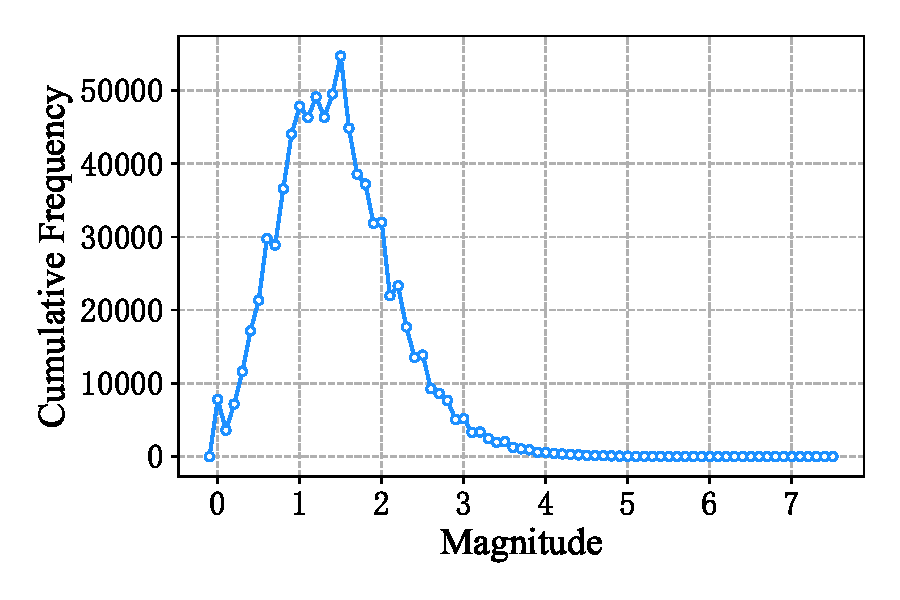
\includegraphics[width=0.60\textwidth]{Img/chap6_seism/seism_m_f.pdf}
  \vspace{-0.5cm}
  \bicaption{震级与频度关系图。}{Relationships bettween magnitude and cumulative frequency.}
  \label{fig:seism_m_f}
\end{figure}

在给定的研究区域内,频度和地震事件的震级服从Gutenberg-Richter法则\citep{Gutenberg1994Frequency,Panakkat2007Neural}。该法则的数学表达形式如下:
\begin{equation}
  \label{eq:seism_Gutenberg-Richter}
  \log N=a-bM.
\end{equation}
其中,$N>0$,$N$指震级不小于阈震级$M_c$的地震事件的累积数量。$b$值为斜率,由震级和频度决定。Gutenberg-Richter法则是指,随着震级逐渐增大,地震频度出现指数级下降\citep{Asim2018Earthquake}。图\ref{fig:seism_m_f}绘制了南加州地区震级与频度关系图,发现小震发生的次数远超出大震,但震级在小于2时,图\ref{fig:seism_m_f}并不满足Gutenberg-Richter法则,因此小震存在缺失的情况。

公式\ref{eq:seism_Gutenberg-Richter}可知,$b$值有助于震级的预测。$b$值不仅能够反映研究区域的地质构造,还能够反映地球物理特性。$b$值一般可以通过两种方法获取,分别为最小二乘(Least Square,简称LS)法和最大似然估计( Maximum Likelihood Estimation,简称MLE)法。图\ref{fig:seism_b_m_1932_2021}绘制了1932年至2021年期间不同起算震级下利用MLE法得到的$b$值。图\ref{fig:seism_logn_m_1932_2021}则绘制了Gutenberg-Richter法则的关系图。图\ref{fig:seism_b_m_1932_2021}和图\ref{fig:seism_logn_m_1932_2021}拐角处的震级可看作是阈震级。综合两图的效果,发现从1932年至2021年期间,南加州地震目录中3级以上的地震基本完备,原始地震目录减少到24,865条。

\begin{figure}[!htbp]
  \centering
  \begin{subfigure}[b]{0.4\textwidth}
    \caption{$b$值与起算震级的关系} 
    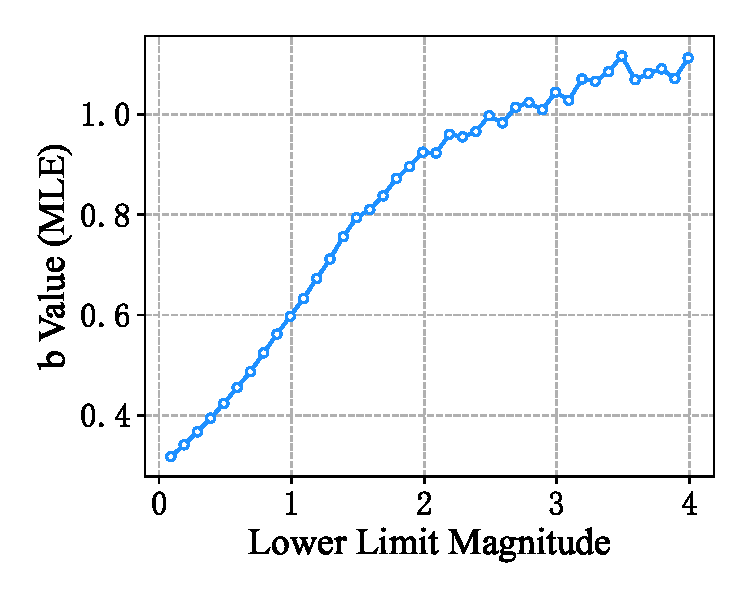
\includegraphics[width=\textwidth]{Img/chap6_seism/seism_b_1932_2021.pdf}
    \label{fig:seism_b_m_1932_2021}
  \end{subfigure}   
  ~
  \begin{subfigure}[b]{0.4\textwidth}
      \caption{$\log N=a-bM$}
      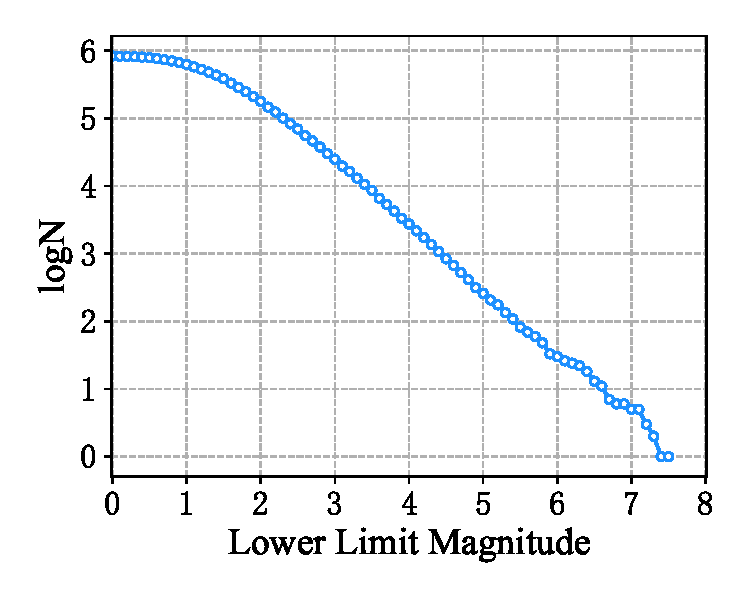
\includegraphics[width=\textwidth]{Img/chap6_seism/seism_logN_1932_2021.pdf}
      \label{fig:seism_logn_m_1932_2021}
  \end{subfigure}
  \vspace{-1cm}
  \bicaption{(a)1932年至2021年期间不同起算震级下利用MLE计算的$b$值;(b)1932年至2021年期间Gutenberg-Richter关系式$\log N=a-bM$。}{(a) The $b$ value calculated by MLE between 1932 and 2021; (b) The Gutenberg-Richter relation $\log N=a-bM$ between 1932 and 2021.}
  \label{fig:seism_mc_1932_2021}
\end{figure}

% 考虑到南加州地震目录前50年有小震缺失的情况。为了更好地利用后四十年的小震数据,我们还对1980年后地震目录记录的完备性检验。通过完备性检验,了解小震缺失对模型的影响。如果证实小震缺失不会对模型有太大的影响,可以适度减小阈震级,使用含更小震级、更长时间的地震目录;若小震会模型性能的稳健性,需要严格遵循小震完备原则。图\ref{fig:seism_b_m_1980_2021}绘制了1932年至2021年期间不同起算震级下利用MLE法得到的$b$值。图\ref{fig:seism_logn_m_1932_2021}则绘制了Gutenberg-Richter法则的关系图。图\ref{fig:seism_logn_m_1980_2021}和图\ref{fig:seism_logn_m_1980_2021}拐角处的震级可看作是阈震级。综合两图的效果,发现从1932年至2021年期间,南加州地震目录中2.2级以上的地震基本完备。

% \begin{figure}[!htbp]
%   \centering
%   \begin{subfigure}[b]{0.4\textwidth}
%     \caption{$b$值与起算震级的关系} 
%     \includegraphics[width=\textwidth]{Img/chap6_seism/seism_b_1980_2021}
%     \label{fig:seism_b_m_1980_2021}
%   \end{subfigure}   
%   ~
%   \begin{subfigure}[b]{0.4\textwidth}
%     \caption{$\log N=a-bM$}
%     \includegraphics[width=\textwidth]{Img/chap6_seism/seism_logN_1980_2021}
%     \label{fig:seism_logn_m_1980_2021}
%   \end{subfigure}
%   \vspace{-1cm}
%   \bicaption{(a)1980年至2021年期间不同起算震级下利用MLE计算的$b$值;(b)1980年至2021年期间Gutenberg-Richter关系式$\log N=a-bM$。}{(a) The $b$ value calculated by MLE between 1980 and 2021; (b) The Gutenberg-Richter relation $\log N=a-bM$ between 1980 and 2021.}
%   \label{fig:seism_mc_1980_2021}
% \end{figure}

\subsection{地震因子}\label{sec:seism_indicator}

本研究的最终目标是预报研究区域内某时间段的最大震级,采取了“以震报震”的策略(基于历史地震目录预报未来最大震级)。但仅仅依靠地震目录预测研究区域内的震级远远不够,我们还需要找出地震目录中隐藏的地质构造背景信息,能够反应地震活动特征的信息,这些信息被我们称作地震因子。因此,地震因子在预报未来震级时至关重要。这些地震因子可以利用地震目录中的数据进行统计计算。

\begin{sidewaystable}[htpb]
  \centering
  \bicaption{基于地震目录的地震因子。}{Indicators related with earthquake catalog.}
  \label{tab:seism_input_data}
  \footnotesize
  \begin{tabular}{llll}
    \toprule
      & 因子 & 公式 & 描述 \\
    \midrule
    1 & $M_{\mathrm{max}}$ &  & 时间窗口内的最大震级 \\ 
    2 & $\mathrm{frequency}$ &  & 地震发生次数 \\ 
    3 & $M_{\mathrm{mean}}$ & $\displaystyle M_{\mathrm{mean}}=\frac{\sum_i{M_i}}{\mathrm{frequency}}$ & 时间窗口内的平均震级 \\ 
    4 & $b_{\mathrm{lstsq}}$ & $\displaystyle b_{\mathrm{lstsq}}=\frac{n\sum_i{(M_i\mathrm{log} N_i)}-\sum_i{M_i}\sum_i\mathrm{log}N_i}{(\sum_i{M_i})^2-n\sum_i{{M_i}^2}}$ & 由最小二乘法计算得到Gutenberg-Richter法则中的$b$值\\
    5 & $b_{\mathrm{mle}}$ & $\displaystyle b_{\mathrm{mle}}=\frac{\mathrm{log}e}{M_{\mathrm{mean}}-M_C}$ & 由最大似然估计法计算得到Gutenberg-Richter法则中的$b$值 \\ 
    6 & $a_{\mathrm{lstsq}}$ & $\displaystyle a_{\mathrm{lstsq}}=\frac{\sum_i{(\mathrm{log}N_i+bM_i)}}{n}$ & 由最小二乘法计算得到Gutenberg-Richter法则中的$a$值 \\ 
    7 & $\Delta M$ & $\displaystyle \Delta M=M_{\mathrm{max, observed}}- \frac{a_{\mathrm{lstsq}}}{b_{\mathrm{lstsq}}}$ & 震级欠缺 \\ 
    8 & $\eta$ & $\displaystyle \eta=\sqrt{\frac{\sum_i{(\mathrm{log} {N_i}}-(a_{\mathrm{lstsq}}-b_{\mathrm{lstsq}}{M_i}))^2}{n}}$ & 基于最小二乘法产生的均方根误差 \\ 
    9 & $\sqrt{E}$ & $\displaystyle \sqrt{E}=\sum_i{\sqrt{E_i}}$, $\displaystyle E_i=10^{11.8+1.5\mathrm{M}_i}.$ & 地震能量平方根\citep{Last2016predicting,asim2017earthquake}  \\ 
    10 & $\mathrm{Lat}_{\mathrm{mean}}$ & $\displaystyle \mathrm{Lat}_{\mathrm{mean}}=\frac{\sum_i{\mathrm{Lat}_i}}{\mathrm{frequency}}$ & 平均纬度 \\ 
    11 & $\mathrm{RMSE}_{\mathrm{Lat}}$ & $\displaystyle \mathrm{RMSE}_{\mathrm{Lat}}=\sqrt{\frac{\sum_i{(\mathrm{Lat}_i-\mathrm{Lat}_\mathrm{mean})}^2}{\mathrm{frequency}}}$ & 纬度的均方根误差 \\ 
    12 & $\mathrm{Lon}_{\mathrm{mean}}$ & $\displaystyle \mathrm{Lon}_{\mathrm{mean}}=\frac{\sum_i{\mathrm{Lon}_i}}{\mathrm{frequency}}$ & 平均经度\\ 
    13 & $\mathrm{RMSE}_{\mathrm{Lon}}$ & $\displaystyle \mathrm{RMSE}_{\mathrm{Lon}}=\sqrt{\frac{\sum_i{(\mathrm{Lon}_i-\mathrm{Lon}_\mathrm{mean})}^2}{\mathrm{frequency}}}$ &  经度的均方根误差 \\ 
    14 & $\mathrm{Lat}_{\sqrt{E}}$ & $\displaystyle \mathrm{Lat}_{\sqrt{E}}=\frac{\sum_i{\mathrm{Lat}_i\sqrt{E_i}}}{\sum_i{\sqrt{E_i}}}$ & 按能量加权计算的震中平均纬度 \\ 
    15 & $\mathrm{Lon}_{\sqrt{E}}$ & $\displaystyle \mathrm{Lon}_{\sqrt{E}}=\frac{\sum_i{\mathrm{Lon}_i\sqrt{E_i}}}{\sum_i{\sqrt{E_i}}}$ & 按能量加权计算的震中平均经度 \\ 
    16 & $k$ & $\mathrm{Lat}=k\mathrm{Lon}+b$ & 由最小二乘法计算得到经纬度之间的斜率 \\
    17 & $M_{\mathrm{future}}$ & & 未来最大震级 \\
    \bottomrule
  \end{tabular} 
\end{sidewaystable}

上节已经提到,$b$值的重要性和计算方法。图\ref{fig:seism_b_lstsq_mle_1932_2021}绘制了$b_{mle}$与$b_{lstsq}$关系图,发现两者的斜率接近于1。在获取$b$值后,也可得到其他几个与$b$值相关的地震因子,例如$a$值、最小二乘法的均方根误差$\eta$、最大震级欠缺$\Delta M$等。表\ref{tab:seism_input_data}描述了17个不同的地震因子,利用前16个因子作为预报最后一个因子。地震因子不仅包括\citet{Panakkat2007Neural}使用的最大震级$M_{\max}$,频度$\mathrm{frequency}$,Giternberg-Richter法则中基于最小二乘法计算得到$a_{\mathrm{lstsq}}$值、$b_{\mathrm{lstsq}}$值、均方根误差$\eta$、最大震级欠缺$\Delta M$、最大似然估计法得到$b_{\mathrm{mle}}$值、地震能量平方根$\sqrt{E}$和平均震级$M_{\mathrm{mean}}$,还包括前人未曾使用的一些新特征。这些新特征包括平均纬度$\mathrm{Lat}_{\mathrm{mean}}$、纬度的均方根误差$\mathrm{RMSE}_{\mathrm{Lat}}$、平均经度$\mathrm{Lon}_{\mathrm{mean}}$、经度的均方根误差$\mathrm{RMSE}_{\mathrm{Lon}}$、按能量加权计算的震中平均纬度$\mathrm{Lat}_{\sqrt{E}}$、按能量加权计算的震中平均经度$\mathrm{Lon}_{\sqrt{E}}$、用最小二乘法计算的经纬度之间的斜率$k$,这7个地震因子能够体现地震发生的空间位置、地震成团或成带分布等。尽管部分因子在一定程度上高度相关,比如$M_{\mathrm{mean}}$与$b_{\mathrm{mle}}$值,$b_{\mathrm{mle}}$值和$b_{\mathrm{lstsq}}$值,$M_{\max}$与$\sqrt{E}$,但研究过程中仍旧保留这些冗余信息,因为机器学习不一定能够很好地捕获这些冗余信息。

\begin{figure}[!htbp]
  \centering
  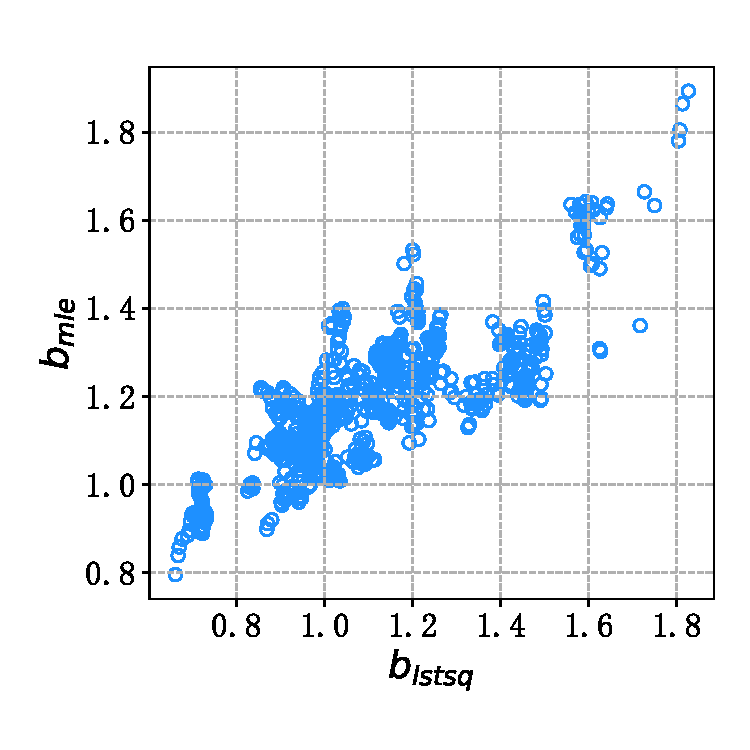
\includegraphics[width=0.60\textwidth]{Img/chap6_seism/seism_b_lstsq_mle_1932_2021.pdf}
  \vspace{-0.5cm}
  \bicaption{$b_{mle}$与$b_{lstsq}$。}{$b_{mle}$ and $b_{lstsq}$.}
  \label{fig:seism_b_lstsq_mle_1932_2021}
\end{figure}

\subsection{时空窗口滑动法}\label{sec:seism_slide}

在第\label{sec:ml_prepare}节,我们已经介绍了窗口滑动法。在探索太阳黑子和泉流量时采取了窗口滑动法,从而将原始观测数据集转化为监督学习数据集。与窗口滑动法有所差异,本章节我们不仅在时间上对数据集进行滑动划分,还包括空间上。这样做的目的是缩小预测震级的区域范围。因为不仅要关注预测震级,还要关注该震级发生的空间范围,而且该范围越小越好。

需要注意的是,部分地震因子的计算是基于统计学基础上的,因此每个时空窗口内地震数目需要达到某个值$N$。如果达不到该值$N$,部分地震因子将会出现极端异常值。为了避免这种情况的出现,将每个时空窗口的地震数限制为至少30个。通常,7级以上的大震前兆会伴有半年至几年不等的前兆信息。因此,为了满足每个时空窗口的地震数至少为30,将时间窗口设为5年,从而空间窗口最小可设为纬度\SI{2}{\degree}\times 经度\SI{4}{\degree}。表\ref{tab:seism_windows_30}展示了每个时空窗口至少有30个地震数的时空窗口信息。

\begin{table}[htpb]
  \bicaption{每个时空窗口至少有30个地震数的时空窗口信息。}{The time and space windows satisfy with 30 earthquake events at least 30.}
  \label{tab:seism_windows_30}
  \centering
  \footnotesize
  \begin{tabular}{cccc}
  \toprule
  \multirow{2}*{时间窗口} & \multirow{2}*{区块序号} & \multicolumn{2}{c}{空间窗口} \\
  \cmidrule(lr){3-4} \noalign{\smallskip}
  & & 纬度范围 & 经度范围 \\
  \midrule
  6年 & 1 & $[35.0N,37.0N]$ & $[114.0W,118.0W]$  \\
      & 2 &  $[35.0N,37.0N]$ & $[118.0W,122.0W]$  \\
      & 3 & $[33.5N,35.5]$ & $[114.0W,118.0W]$  \\
      & 4 & $[33.5N,35.5N]$ & $[117.5W,121.5W]$  \\
      & 5 & $[32.0N,34.0N]$ & $[114.0W,118.0W]$  \\
      & 6 & $[32.0N,34.0N]$ & $[117.0W,121.0W]$  \\
  \bottomrule
  \end{tabular} 
\end{table}

时间窗口按月滑动。空间窗口按照表\ref{tab:seism_windows_30}中区块序号进行滑动,即从研究区域的左上角开始向东滑动\SI{4}{\degree}。到达区域边缘后,再向南滑动\SI{1.5}{\degree}。向南滑动开始时离左边缘\SI{0.5}{\degree}向东滑动\SI{3.5}{\degree}。到达区域边缘后,再此向南滑动\SI{1.5}{\degree}。向南滑动开始时离左边缘\SI{1}{\degree}向东滑动\SI{3}{\degree}。这样重复6次后,一共得到6个空间区块。这划分区块是,西边的区块逐渐右移,这样做的目的是,研究角区域的西南角为海域,地震目录中缺失了这部分的数据。根据时空窗口滑动,前16个地震因子和未来最大震级可被近似表达为:
\begin{equation}
  \label{eq:seism_m_indicator}
  \begin{split}
    M_{\mathrm{future}}^{\mathrm{loc}}(t+T)=F[M_{\mathrm{max}}^{\mathrm{loc}}(t-\Delta),\mathrm{frequency}^{\text{loc}}(t-\Delta),M_{\mathrm{mean}}^{\text{loc}}(t-\Delta),\\
    b_{\mathrm{lstsq}}^{\text{loc}}(t-\Delta),b_{\mathrm{mle}}^{\text{loc}}(t-\Delta),a_{\mathrm{lstsq}}^{\text{loc}}(t-\Delta),\Delta^{\text{loc}}M(t-\Delta),\\
    \eta^{\text{loc}}(t-\Delta),\sqrt{E}^{\text{loc}}(t-\Delta),\mathrm{Lat}_{\mathrm{mean}}^{\text{loc}}(t-\Delta),\mathrm{RMSE}_{\mathrm{Lat}}^{\text{loc}}(t-\Delta),\\
    \mathrm{Lon}_{\mathrm{mean}}^{\text{loc}}(t-\Delta),\mathrm{RMSE}_{\mathrm{Lon}}^{\text{loc}}(t-\Delta),\mathrm{Lat}^{\text{loc}}_{\sqrt{E}}(t-\Delta),\\
    \mathrm{Lon}^{\text{loc}}_{\sqrt{E}}(t-\Delta),k^{\text{loc}}(t-\Delta),M_{\mathrm{future}}^{\text{loc}}(t-\Delta)]
  \end{split}
\end{equation}
其中,$t$代表当前时刻,$-\Delta$代表历史时间窗口(即输入时间窗口),$+T$代表未来时间窗口(即输出时间窗口),$\text{loc}$代表区块序号,$\text{loc}\in\{1,2,\ldots,6\}$。$M_{\mathrm{future}}^{\text{loc}}(t+T)$代表未来时间窗口$+T$内第$\text{loc}$个区块的最大震级。$M_{\mathrm{max}}^{\mathrm{loc}}(t-\Delta)$代表历史时间窗口$-\Delta$内第$\text{loc}$个区块的最大震级。其他变量的含义以此类推。式\ref{eq:seism_m_indicator}明确指出,模型的输入是历史记录的16个地震因子在6个不同区块的统计值,输出为未来时间窗口内的最大震级。图\ref{fig:seism_magnitude_index_1932_2021}绘制了不同区块未来一年最大震级时间序列图。从图\ref{fig:seism_magnitude_index_1932_2021}得知,该地区最大震级不超过8,未来一年最大震级多数位于3.5至5.5之间。

\begin{figure}[!htbp]
  \centering
  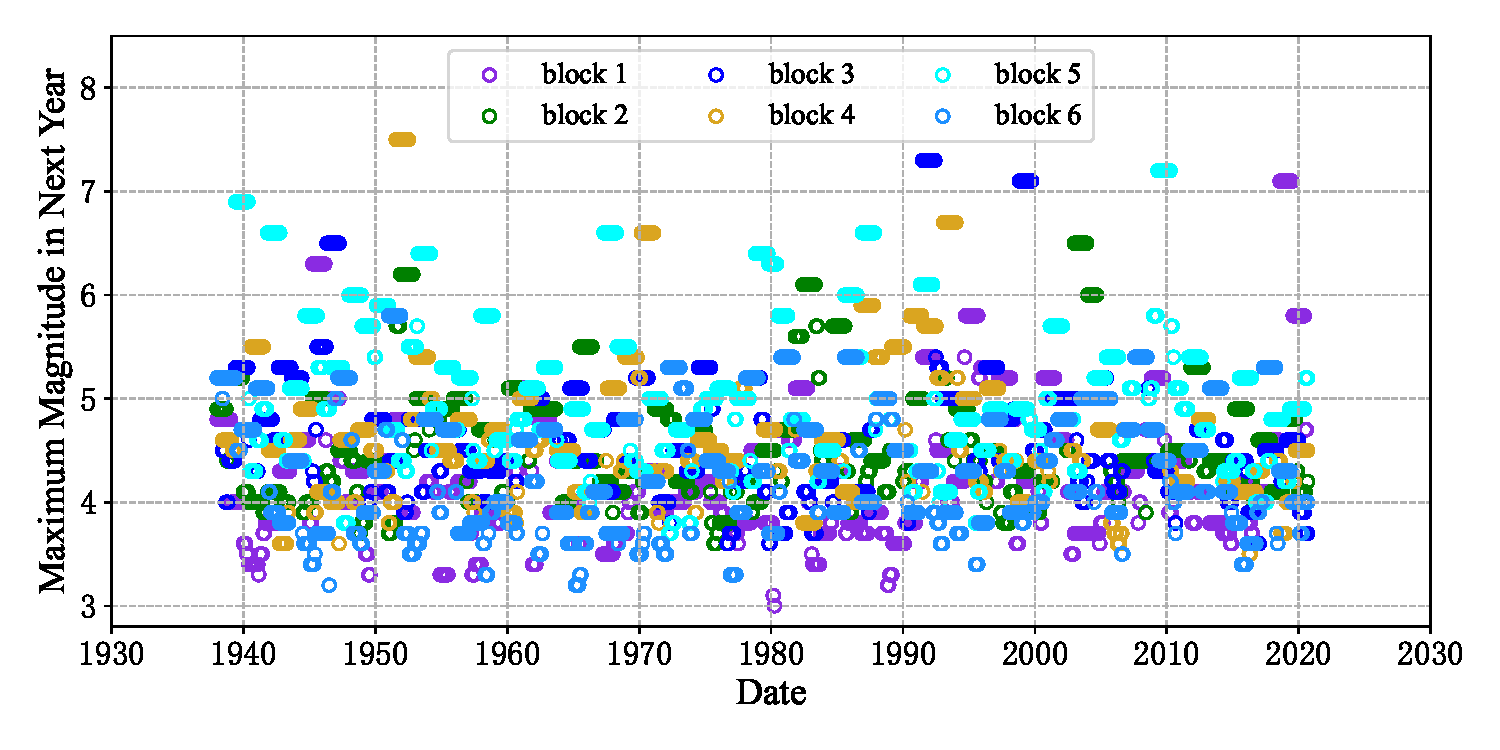
\includegraphics[width=0.60\textwidth]{Img/chap6_seism/seism_magnitude_index_1932_2021.pdf}
  \vspace{-0.5cm}
  \bicaption{不同区块未来一年最大震级时间序列图。}{Time series of the maximum magnitude in mext year with different blocks.}
  \label{fig:seism_magnitude_index_1932_2021}
\end{figure}

通过时空滑动窗口法,我们可以将原始数据集$D_{\text{raw}}$转换为监督学习数据集$D_{\text{supervised}}$。紧接着,我们将数据集$D_{\text{supervised}}$分割为训练集$D_{\text{train}}$和测试集$D_{\text{test}}$,分割比例为0.8:0.2。在训练集$D_{\text{train}}$和测试集$D_{\text{test}}$被使用之前,我们需要对两者分别进行归一化处理(第\ref{sec:ml_scaler}节),得到了训练集$D^T_{\text{train}}$和测试集$D^T_{\text{test}}$。

\section{结果分析}\label{sec:seism_result}

这里,我们采取了8中不同类型的模型,分别为LSTM-RNN、SVR、LR、RF、DT、KN、GBR、ETR。各种模型输入则是6个区块在某个特定时刻前6年时间窗口内的16个预报因子,即输入层为$6\times 16=96$个节点,输出是某个区块下一年的最大震级。

% 从表\ref{tab:seism_block1}至表\ref{tab:seism_block6}中LSTM-RNN的表现来看,两层的LSTM-RNN在隐藏层节点数为32、64、128均出现了很大程度的过拟合现象。可见LSTM-RNN网络相对于本数据集而言,过于复杂,因此这里我们使用其他几种机器学习方法,仍然发现了很大程度的过拟合现象。从这些结果可以看出,机器学习对南加州地区的地震中期预报是失败的。

% \begin{table}[!htbp]
%     \bicaption{不同模型预报区块1未来一年最大震级的拟合指标效果。}{The metrics for predicting the maximum magnitute of block 1 in next year by different models.}
%     \label{tab:seism_block1}
%     \centering
%     \footnotesize
%     \begin{tabular}{clcccc}
%         \toprule
%         \multirow{2}*{模型} &
%          \multirow{2}*{\makecell[{l}{p{3cm}}]{输入/隐藏层节点\\数/过滤器数}} & \multicolumn{2}{c}{训练集} & \multicolumn{2}{c}{验证集}\\
%         \cmidrule(lr){3-4}\cmidrule(lr){5-6} \noalign{\smallskip}
%          & & MSE & RMSE & MSE & RMSE\\
%         \midrule
%         LSTM & 32(LSTM) & 0.0053 & 0.0731 & 0.1138 & 0.3374  \\
%         & 64(LSTM) & 0.0050 & 0.0708 & 0.0620 & 0.2490 \\
%         & 128(LSTM) & 0.0097 & 0.0984 & 0.0913 & 0.3022
%         \\ \hline
%         SVR & & 0.0067 & 0.0820 & 0.1725 & 0.4153\\
%         LR & & 0.0053 & 0.0728 & 0.1540 & 0.3924\\
%         RF & & 0.0013 & 0.0362 & 0.0699 & 0.2644 \\
%         DT & & 0.0000 & 0.0000 & 0.1082 & 0.3290 \\
%         KN & & 0.0000 & 0.0000 & 0.1080 & 0.3286 \\
%         GBR & & 0.0013 & 0.0354 & 0.0907 & 0.3012 \\
%         ETR & & 0.0000 & 0.0000 & 0.1068 & 0.3268 \\
%         % \hline
%         \bottomrule
%     \end{tabular}
% \end{table}

% \begin{figure}[!htbp]
% \center
%     \begin{overpic}[width=0.48\textwidth]{seism-lstm-min_year1932-max_year2021-span_lat2-span_lon4-time_window72-next_month12-min_mag3-layer2-layer_size64-loc_block1-PredictM}\put(0,40){(a)}\end{overpic}
%     \begin{overpic}[width=0.48\textwidth]{seism-svr-min_year1932-max_year2021-span_lat2-span_lon4-time_window72-next_month12-min_mag3-layer2-layer_size128-loc_block1-PredictM}\put(0,40){(b)}\end{overpic} \\
%     \begin{overpic}[width=0.48\textwidth]{seism-lr-min_year1932-max_year2021-span_lat2-span_lon4-time_window72-next_month12-min_mag3-layer2-layer_size128-loc_block1-PredictM}\put(0,40){(c)}\end{overpic}
%     \begin{overpic}[width=0.48\textwidth]{seism-rf-min_year1932-max_year2021-span_lat2-span_lon4-time_window72-next_month12-min_mag3-layer2-layer_size128-loc_block1-PredictM}\put(0,40){(d)}\end{overpic} \\
%     \begin{overpic}[width=0.48\textwidth]{seism-dt-min_year1932-max_year2021-span_lat2-span_lon4-time_window72-next_month12-min_mag3-layer2-layer_size128-loc_block1-PredictM}\put(0,40){(e)}\end{overpic}
%     \begin{overpic}[width=0.48\textwidth]{seism-kn-min_year1932-max_year2021-span_lat2-span_lon4-time_window72-next_month12-min_mag3-layer2-layer_size128-loc_block1-PredictM}\put(0,40){(f)}\end{overpic} \\
%     \begin{overpic}[width=0.48\textwidth]{seism-gbr-min_year1932-max_year2021-span_lat2-span_lon4-time_window72-next_month12-min_mag3-layer2-layer_size128-loc_block1-PredictM}\put(0,40){(g)}\end{overpic}
%     \begin{overpic}[width=0.48\textwidth]{seism-etr-min_year1932-max_year2021-span_lat2-span_lon4-time_window72-next_month12-min_mag3-layer2-layer_size128-loc_block1-PredictM}\put(0,40){(h)}\end{overpic}
%     \bicaption{不同模型预报区块1未来一年最大震级的预报效果。}{The effects of predicting the maximum magnitute of block 1 in next year by different models.}
%     \label{fig:seism-min_year1932-max_year2021-span_lat2-span_lon4-time_window72-next_month12-min_mag3-layer2-layer_size128-loc_block1-PredictM}
% \end{figure}


% \begin{table}[!htbp]
%     \bicaption{不同模型预报区块2未来一年最大震级的拟合指标效果。}{The metrics for predicting the maximum magnitute of block 2 in next year by different models.}
%     \label{tab:seism_block2}
%     \centering
%     \footnotesize
%     \begin{tabular}{clcccc}
%         \toprule
%         \multirow{2}*{模型} &
%          \multirow{2}*{\makecell[{l}{p{3cm}}]{输入/隐藏层节点\\数/过滤器数}} & \multicolumn{2}{c}{训练集} & \multicolumn{2}{c}{验证集}\\
%         \cmidrule(lr){3-4}\cmidrule(lr){5-6} \noalign{\smallskip}
%          & & MSE & RMSE & MSE & RMSE\\
%         \midrule
%         LSTM & 32(LSTM) & 0.0121 & 0.1102 & 0.0392 & 0.1979 \\
%         & 64(LSTM) & 0.0089 & 0.0941 & 0.0656 & 0.2561 \\
%         & 128(LSTM) & 0.0095 & 0.0977 & 0.0781 & 0.2795
%         \\ \hline
%         SVR & & 0.0067 & 0.0820 & 0.1725 & 0.4153\\
%         LR & & 0.0053 & 0.0728 & 0.1540 & 0.3924\\
%         RF & & 0.0013 & 0.0362 & 0.0699 & 0.2644 \\
%         DT & & 0.0000 & 0.0000 & 0.1082 & 0.3290 \\
%         KN & & 0.0000 & 0.0000 & 0.1080 & 0.3286 \\
%         GBR & & 0.0013 & 0.0354 & 0.0907 & 0.3012 \\
%         ETR & & 0.0000 & 0.0000 & 0.1068 & 0.3268 \\
%         % \hline
%         \bottomrule
%     \end{tabular}
% \end{table}

% \begin{figure}[!htbp]
% \center
%     \begin{overpic}[width=0.48\textwidth]{seism-lstm-min_year1932-max_year2021-span_lat2-span_lon4-time_window72-next_month12-min_mag3-layer2-layer_size32-loc_block2-PredictM}\put(0,40){(a)}\end{overpic}
%     \begin{overpic}[width=0.48\textwidth]{seism-svr-min_year1932-max_year2021-span_lat2-span_lon4-time_window72-next_month12-min_mag3-layer2-layer_size128-loc_block2-PredictM}\put(0,40){(b)}\end{overpic} \\
%     \begin{overpic}[width=0.48\textwidth]{seism-lr-min_year1932-max_year2021-span_lat2-span_lon4-time_window72-next_month12-min_mag3-layer2-layer_size128-loc_block2-PredictM}\put(0,40){(c)}\end{overpic}
%     \begin{overpic}[width=0.48\textwidth]{seism-rf-min_year1932-max_year2021-span_lat2-span_lon4-time_window72-next_month12-min_mag3-layer2-layer_size128-loc_block2-PredictM}\put(0,40){(d)}\end{overpic} \\
%     \begin{overpic}[width=0.48\textwidth]{seism-dt-min_year1932-max_year2021-span_lat2-span_lon4-time_window72-next_month12-min_mag3-layer2-layer_size128-loc_block2-PredictM}\put(0,40){(e)}\end{overpic}
%     \begin{overpic}[width=0.48\textwidth]{seism-kn-min_year1932-max_year2021-span_lat2-span_lon4-time_window72-next_month12-min_mag3-layer2-layer_size128-loc_block2-PredictM}\put(0,40){(f)}\end{overpic} \\
%     % \begin{overpic}[width=0.48\textwidth]{seism-gbr-min_year1932-max_year2021-span_lat2-span_lon4-time_window72-next_month12-min_mag3-layer2-layer_size128-loc_block2-PredictM}\put(0,40){(g)}\end{overpic}
%     \begin{overpic}[width=0.48\textwidth]{seism-etr-min_year1932-max_year2021-span_lat2-span_lon4-time_window72-next_month12-min_mag3-layer2-layer_size128-loc_block2-PredictM}\put(0,40){(h)}\end{overpic}
%     \bicaption{不同模型预报区块2未来一年最大震级的预报效果。}{The effects of predicting the maximum magnitute of block 2 in next year by different models.}
%     \label{fig:seism-min_year1932-max_year2021-span_lat2-span_lon4-time_window72-next_month12-min_mag3-layer2-layer_size128-loc_block2-PredictM}
% \end{figure}


% \begin{table}[!htbp]
%     \bicaption{不同模型预报区块3未来一年最大震级的拟合指标效果。}{The metrics for predicting the maximum magnitute of block 3 in next year by different models.}
%     \label{tab:seism_block3}
%     \centering
%     \footnotesize
%     \begin{tabular}{clcccc}
%         \toprule
%         \multirow{2}*{模型} &
%          \multirow{2}*{\makecell[{l}{p{3cm}}]{输入/隐藏层节点\\数/过滤器数}} & \multicolumn{2}{c}{训练集} & \multicolumn{2}{c}{验证集}\\
%         \cmidrule(lr){3-4}\cmidrule(lr){5-6} \noalign{\smallskip}
%          & & MSE & RMSE & MSE & RMSE\\
%         \midrule
%         LSTM & 32(LSTM) & 0.0080 & 0.0893 & 0.0993 & 0.3150 \\
%         & 64(LSTM) & 0.0150 & 0.1226 & 0.2917 & 0.5401 \\
%         & 128(LSTM) & 0.0064 & 0.0800 & 0.1468 & 0.3832
%         \\ \hline
%         SVR & & 0.0126 & 0.1122 & 0.2169 & 0.4657 \\
%         LR & & 0.0088 & 0.0936 & 0.2144 & 0.4631 \\
%         RF & & 0.0017 & 0.0415 & 0.0668 & 0.2584 \\
%         DT & & 0.0000 & 0.0000 & 0.0471 & 0.2170 \\
%         KN & & 0.0000 & 0.0000 & 0.1088 & 0.3299 \\
%         GBR & & 0.0019 & 0.0436 & 0.0560 & 0.2366 \\
%         ETR & & 0.0000 & 0.0000 & 0.1039 & 0.3223 \\
%         \bottomrule
%     \end{tabular}
% \end{table}

% \begin{figure}[!htbp]
% \center
%     \begin{overpic}[width=0.48\textwidth]{seism-lstm-min_year1932-max_year2021-span_lat2-span_lon4-time_window72-next_month12-min_mag3-layer2-layer_size32-loc_block3-PredictM}\put(0,40){(a)}\end{overpic}
%     \begin{overpic}[width=0.48\textwidth]{seism-svr-min_year1932-max_year2021-span_lat2-span_lon4-time_window72-next_month12-min_mag3-layer2-layer_size128-loc_block3-PredictM}\put(0,40){(b)}\end{overpic} \\
%     \begin{overpic}[width=0.48\textwidth]{seism-lr-min_year1932-max_year2021-span_lat2-span_lon4-time_window72-next_month12-min_mag3-layer2-layer_size128-loc_block3-PredictM}\put(0,40){(c)}\end{overpic}
%     \begin{overpic}[width=0.48\textwidth]{seism-rf-min_year1932-max_year2021-span_lat2-span_lon4-time_window72-next_month12-min_mag3-layer2-layer_size128-loc_block3-PredictM}\put(0,40){(d)}\end{overpic} \\
%     \begin{overpic}[width=0.48\textwidth]{seism-dt-min_year1932-max_year2021-span_lat2-span_lon4-time_window72-next_month12-min_mag3-layer2-layer_size128-loc_block3-PredictM}\put(0,40){(e)}\end{overpic}
%     \begin{overpic}[width=0.48\textwidth]{seism-kn-min_year1932-max_year2021-span_lat2-span_lon4-time_window72-next_month12-min_mag3-layer2-layer_size128-loc_block3-PredictM}\put(0,40){(f)}\end{overpic} \\
%     \begin{overpic}[width=0.48\textwidth]{seism-gbr-min_year1932-max_year2021-span_lat2-span_lon4-time_window72-next_month12-min_mag3-layer2-layer_size128-loc_block3-PredictM}\put(0,40){(g)}\end{overpic}
%     \begin{overpic}[width=0.48\textwidth]{seism-etr-min_year1932-max_year2021-span_lat2-span_lon4-time_window72-next_month12-min_mag3-layer2-layer_size128-loc_block3-PredictM}\put(0,40){(h)}\end{overpic}
%     \bicaption{不同模型预报区块3未来一年最大震级的预报效果。}{The effects of predicting the maximum magnitute of block 3 in next year by different models.}
%     \label{fig:seism-min_year1932-max_year2021-span_lat2-span_lon4-time_window72-next_month12-min_mag3-layer2-layer_size128-loc_block3-PredictM}
% \end{figure}



% \begin{table}[!htbp]
%     \bicaption{不同模型预报区块4未来一年最大震级的拟合指标效果。}{The metrics for predicting the maximum magnitute of block 4 in next year by different models.}
%     \label{tab:seism_block4}
%     \centering
%     \footnotesize
%     \begin{tabular}{clcccc}
%         \toprule
%         \multirow{2}*{模型} &
%          \multirow{2}*{\makecell[{l}{p{3cm}}]{输入/隐藏层节点\\数/过滤器数}} & \multicolumn{2}{c}{训练集} & \multicolumn{2}{c}{验证集}\\
%         \cmidrule(lr){3-4}\cmidrule(lr){5-6} \noalign{\smallskip}
%          & & MSE & RMSE & MSE & RMSE\\
%         \midrule
%         LSTM & 32(LSTM) & 0.0085 & 0.0924 & 0.0284 & 0.1685 \\
%         & 64(LSTM) & 0.0067 & 0.0817 & 0.0300 & 0.1732  \\
%         & 128(LSTM) & 0.0077 & 0.0879 & 0.0268 & 0.1639
%         \\ \hline
%         SVR & & 0.0116 & 0.1077 & 0.0347 & 0.1864 \\
%         LR & & 0.0076 & 0.0875 & 0.0959 & 0.3097 \\
%         RF & & 0.0016 & 0.0405 & 0.0652 & 0.2553 \\
%         DT & & 0.0000 & 0.0000 & 0.0190 & 0.1380 \\
%         KN & & 0.0000 & 0.0000 & 0.0172 & 0.1310 \\
%         GBR & & 0.0018 & 0.0428 & 0.0174 & 0.1319 \\
%         ETR & & 0.0000 & 0.0000 & 0.0287 & 0.1695 \\
%         \bottomrule
%     \end{tabular}
% \end{table}

% \begin{figure}[!htbp]
% \center
%     \begin{overpic}[width=0.48\textwidth]{seism-lstm-min_year1932-max_year2021-span_lat2-span_lon4-time_window72-next_month12-min_mag3-layer2-layer_size128-loc_block4-PredictM}\put(0,40){(a)}\end{overpic}
%     \begin{overpic}[width=0.48\textwidth]{seism-svr-min_year1932-max_year2021-span_lat2-span_lon4-time_window72-next_month12-min_mag3-layer2-layer_size64-loc_block4-PredictM}\put(0,40){(b)}\end{overpic} \\
%     \begin{overpic}[width=0.48\textwidth]{seism-lr-min_year1932-max_year2021-span_lat2-span_lon4-time_window72-next_month12-min_mag3-layer2-layer_size64-loc_block4-PredictM}\put(0,40){(c)}\end{overpic}
%     \begin{overpic}[width=0.48\textwidth]{seism-rf-min_year1932-max_year2021-span_lat2-span_lon4-time_window72-next_month12-min_mag3-layer2-layer_size64-loc_block4-PredictM}\put(0,40){(d)}\end{overpic} \\
%     \begin{overpic}[width=0.48\textwidth]{seism-dt-min_year1932-max_year2021-span_lat2-span_lon4-time_window72-next_month12-min_mag3-layer2-layer_size64-loc_block4-PredictM}\put(0,40){(e)}\end{overpic}
%     \begin{overpic}[width=0.48\textwidth]{seism-kn-min_year1932-max_year2021-span_lat2-span_lon4-time_window72-next_month12-min_mag3-layer2-layer_size64-loc_block4-PredictM}\put(0,40){(f)}\end{overpic} \\
%     \begin{overpic}[width=0.48\textwidth]{seism-gbr-min_year1932-max_year2021-span_lat2-span_lon4-time_window72-next_month12-min_mag3-layer2-layer_size64-loc_block4-PredictM}\put(0,40){(g)}\end{overpic}
%     \begin{overpic}[width=0.48\textwidth]{seism-etr-min_year1932-max_year2021-span_lat2-span_lon4-time_window72-next_month12-min_mag3-layer2-layer_size64-loc_block4-PredictM}\put(0,40){(h)}\end{overpic}
%     \bicaption{不同模型预报区块4未来一年最大震级的预报效果。}{The effects of predicting the maximum magnitute of block 4 in next year by different models. }
%     \label{fig:seism-min_year1932-max_year2021-span_lat2-span_lon4-time_window72-next_month12-min_mag3-layer2-layer_size64-loc_block4-PredictM}
% \end{figure}


% \begin{table}[!htbp]
%     \bicaption{不同模型预报区块5未来一年最大震级的拟合指标效果。}{The metrics for predicting the maximum magnitute of block 5 in next year by different models.}
%     \label{tab:seism_block5}
%     \centering
%     \footnotesize
%     \begin{tabular}{clcccc}
%         \toprule
%         \multirow{2}*{模型} &
%          \multirow{2}*{\makecell[{l}{p{3cm}}]{输入/隐藏层节点\\数/过滤器数}} & \multicolumn{2}{c}{训练集} & \multicolumn{2}{c}{验证集}\\
%         \cmidrule(lr){3-4}\cmidrule(lr){5-6} \noalign{\smallskip}
%          & & MSE & RMSE & MSE & RMSE\\
%         \midrule
%         LSTM & 32(LSTM) & 0.0144 & 0.1202 & 0.2001 & 0.4474 \\
%         & 64(LSTM) & 0.0122 & 0.1105 & 0.2739 & 0.5233  \\
%         & 128(LSTM) & 0.0121 & 0.1102 & 0.2729 & 0.5224
%         \\ \hline
%         SVR & & 0.0209 & 0.1447 & 0.3093 & 0.5561 \\
%         LR & & 0.0139 & 0.1180 & 0.8346 & 0.9135 \\
%         RF & & 0.0030 & 0.0546 & 0.0277 & 0.1664 \\
%         DT & & 0.0000 & 0.0000 & 0.0511 & 0.2259 \\
%         KN & & 0.0000 & 0.0000 & 0.0620 & 0.2490 \\
%         GBR & & 0.0032 & 0.0565 & 0.0593 & 0.2435 \\
%         ETR & & 0.0000 & 0.0000 & 0.2238 & 0.4731 \\
%         \bottomrule
%     \end{tabular}
% \end{table}

% \begin{figure}[!htbp]
% \center
%     \begin{overpic}[width=0.48\textwidth]{seism-lstm-min_year1932-max_year2021-span_lat2-span_lon4-time_window72-next_month12-min_mag3-layer2-layer_size32-loc_block5-PredictM}\put(0,40){(a)}\end{overpic}
%     \begin{overpic}[width=0.48\textwidth]{seism-svr-min_year1932-max_year2021-span_lat2-span_lon4-time_window72-next_month12-min_mag3-layer2-layer_size64-loc_block5-PredictM}\put(0,40){(b)}\end{overpic} \\
%     \begin{overpic}[width=0.48\textwidth]{seism-lr-min_year1932-max_year2021-span_lat2-span_lon4-time_window72-next_month12-min_mag3-layer2-layer_size64-loc_block5-PredictM}\put(0,40){(c)}\end{overpic}
%     \begin{overpic}[width=0.48\textwidth]{seism-rf-min_year1932-max_year2021-span_lat2-span_lon4-time_window72-next_month12-min_mag3-layer2-layer_size64-loc_block5-PredictM}\put(0,40){(d)}\end{overpic} \\
%     \begin{overpic}[width=0.48\textwidth]{seism-dt-min_year1932-max_year2021-span_lat2-span_lon4-time_window72-next_month12-min_mag3-layer2-layer_size64-loc_block5-PredictM}\put(0,40){(e)}\end{overpic}
%     \begin{overpic}[width=0.48\textwidth]{seism-kn-min_year1932-max_year2021-span_lat2-span_lon4-time_window72-next_month12-min_mag3-layer2-layer_size64-loc_block5-PredictM}\put(0,40){(f)}\end{overpic} \\
%     \begin{overpic}[width=0.48\textwidth]{seism-gbr-min_year1932-max_year2021-span_lat2-span_lon4-time_window72-next_month12-min_mag3-layer2-layer_size64-loc_block5-PredictM}\put(0,40){(g)}\end{overpic}
%     \begin{overpic}[width=0.48\textwidth]{seism-etr-min_year1932-max_year2021-span_lat2-span_lon4-time_window72-next_month12-min_mag3-layer2-layer_size64-loc_block5-PredictM}\put(0,40){(h)}\end{overpic}
%     \bicaption{不同模型预报区块5未来一年最大震级的预报效果。}{The effects of predicting the maximum magnitute of block 5 in next year by different models. }
%     \label{fig:seism-min_year1932-max_year2021-span_lat2-span_lon4-time_window72-next_month12-min_mag3-layer2-layer_size64-loc_block5-PredictM}
% \end{figure}


% \begin{table}[!htbp]
%     \bicaption{不同模型预报区块6未来一年最大震级的拟合指标效果。}{The metrics for predicting the maximum magnitute of block 6 in next year by different models.}
%     \label{tab:seism_block6}
%     \centering
%     \footnotesize
%     \begin{tabular}{clcccc}
%         \toprule
%         \multirow{2}*{模型} &
%          \multirow{2}*{\makecell[{l}{p{3cm}}]{输入/隐藏层节点\\数/过滤器数}} & \multicolumn{2}{c}{训练集} & \multicolumn{2}{c}{验证集}\\
%         \cmidrule(lr){3-4}\cmidrule(lr){5-6} \noalign{\smallskip}
%          & & MSE & RMSE & MSE & RMSE\\
%         \midrule
%         LSTM & 32(LSTM) & 0.0146 & 0.1208 & 0.0510 & 0.2257 \\
%         & 64(LSTM) & 0.0170 & 0.1305 & 0.0816 & 0.2856 \\
%         & 128(LSTM) & 0.0157 & 0.1254 & 0.0615 & 0.2480
%         \\ \hline
%         SVR & & 0.0240 & 0.1549 & 0.0578 & 0.2404 \\
%         LR & & 0.0161 & 0.1267 & 0.2658 & 0.5155 \\
%         RF & & 0.0035 & 0.0592 & 0.0624 & 0.2498 \\
%         DT & & 0.0000 & 0.0000 & 0.0831 & 0.2883 \\
%         KN & & 0.0000 & 0.0000 & 0.1124 & 0.3353 \\
%         GBR & & 0.0039 & 0.0625 & 0.0598 & 0.2446 \\
%         ETR & & 0.0000 & 0.0000 & 0.0539 & 0.2322 \\
%         \bottomrule
%     \end{tabular}
% \end{table}

% \begin{figure}[!htbp]
% \center
%     \begin{overpic}[width=0.48\textwidth]{seism-lstm-min_year1932-max_year2021-span_lat2-span_lon4-time_window72-next_month12-min_mag3-layer2-layer_size32-loc_block6-PredictM}\put(0,40){(a)}\end{overpic}
%     \begin{overpic}[width=0.48\textwidth]{seism-svr-min_year1932-max_year2021-span_lat2-span_lon4-time_window72-next_month12-min_mag3-layer2-layer_size64-loc_block6-PredictM}\put(0,40){(b)}\end{overpic} \\
%     \begin{overpic}[width=0.48\textwidth]{seism-lr-min_year1932-max_year2021-span_lat2-span_lon4-time_window72-next_month12-min_mag3-layer2-layer_size64-loc_block6-PredictM}\put(0,40){(c)}\end{overpic}
%     \begin{overpic}[width=0.48\textwidth]{seism-rf-min_year1932-max_year2021-span_lat2-span_lon4-time_window72-next_month12-min_mag3-layer2-layer_size64-loc_block6-PredictM}\put(0,40){(d)}\end{overpic} \\
%     \begin{overpic}[width=0.48\textwidth]{seism-dt-min_year1932-max_year2021-span_lat2-span_lon4-time_window72-next_month12-min_mag3-layer2-layer_size64-loc_block6-PredictM}\put(0,40){(e)}\end{overpic}
%     \begin{overpic}[width=0.48\textwidth]{seism-kn-min_year1932-max_year2021-span_lat2-span_lon4-time_window72-next_month12-min_mag3-layer2-layer_size64-loc_block6-PredictM}\put(0,40){(f)}\end{overpic} \\
%     \begin{overpic}[width=0.48\textwidth]{seism-gbr-min_year1932-max_year2021-span_lat2-span_lon4-time_window72-next_month12-min_mag3-layer2-layer_size64-loc_block6-PredictM}\put(0,40){(g)}\end{overpic}
%     \begin{overpic}[width=0.48\textwidth]{seism-etr-min_year1932-max_year2021-span_lat2-span_lon4-time_window72-next_month12-min_mag3-layer2-layer_size64-loc_block6-PredictM}\put(0,40){(h)}\end{overpic}
%     \bicaption{不同模型预报区块6未来一年最大震级的预报效果。}{The effects of predicting the maximum magnitute of block 6 in next year by different models. }
%     \label{fig:seism-min_year1932-max_year2021-span_lat2-span_lon4-time_window72-next_month12-min_mag3-layer2-layer_size64-loc_block6-PredictM}
% \end{figure}


\section{讨论与结论}\label{sec:seism_conclusion}

% 这里我们需要再次说明欠拟合和过拟合。欠拟合(under-fitting)也称欠学习,它的直观表现是算法训练得到的模型在训练集上表现差,未学到数据的规律。引起欠拟合的原因可能有:
% \begin{enumerate}
%     \item 模型本身过于简单,例如数据本身是非线性的,但使用了线性模型;
%     \item 特征数太少无法正确的建立统计关系。
% \end{enumerate}

% 过拟合(over-fitting)也称过学习,它的直观表现是算法在训练集上表现好,但在测试集上表现不好,泛化性能差。过拟合是在模型参数拟合过程中由于训练数据包含抽样误差,在训练时复杂的模型将抽样误差也进行了拟合。所谓抽样误差,是指抽样得到的样本集和整体数据集之间的偏差。直观来看,引起过拟合的可能原因有:
% \begin{enumerate}
%     \item 模型本身过于复杂,以至于拟合了训练样本集中的噪声。此时需要选用更简单的模型,或者对模型进行简化;
%     \item 训练样本太少或者缺乏代表性。此时需要增加样本数,或者增加样本的多样性;
%     \item 训练样本噪声的干扰,导致模型拟合了这些噪声,这时需要剔除噪声数据或者改用对噪声不敏感的模型。
% \end{enumerate}

% 过拟合是有监督的机器学习算法长期以来需要面临的一个问题。下表给出了实际应用时判断过拟合与欠拟合的准则:
% \begin{table}[!htbp]
%     \bicaption{过拟合与欠拟合的判断标准。}{The criterion for under-fitting and over-fitting.}
%     \label{tab:seism_overfit}
%     \centering
%     \footnotesize
%     \begin{tabular}{ccc}
%         \toprule
%         训练集上的表现 & 测试集上的表现 & 判断 \\
%         \midrule
%         欠佳 & 欠佳 & 欠拟合 \\
%         好 & 欠佳 & 过拟合 \\
%         好 & 好 & 适度拟合 \\
%         \bottomrule
%     \end{tabular}
% \end{table}

% 当然,我们也可以从偏差和方差的角度来看待欠拟合和过拟合。模型的泛化误差来源于三部分,即偏差(bias)、方差(variance)和噪音(noise)。偏差度量了学习算法的期望预报值与真实值的偏离程度,即刻画了学习算法本身的拟合能力。假设地震因子特征向量为$\Vector{X}$,输出震级为$M$,实际震级为$M^{\prime}$,要拟合的目标函数为$f(\Vector{X})$,训练的函数为$\hat{f}(\Vector{X})$,则偏差为:
% \begin{equation}
%   \mathrm{Bais}^2[\Vector{X}]=(\hat{f}(\Vector{X})-M)^2.
% \end{equation}
% 根据该定义,高偏差意味着模型本身的输出值与期望值差距大,因此会导致欠拟合的问题。

% 与偏差不同,方差度量了同样大小的训练集的变动导致学习性能的变化,即刻画了数据扰动所造成的影响。它是训练样本的小波动敏感而导致的误差。方差可以理解为模型预报值的变化范围,即模型预报值的波动程度。根据概率论中方差的定义,有:
% \begin{equation}
%   \mathrm{Variance}[\Vector{X}]=E[(\hat{f}(\Vector{X})-f(\Vector{X}))^2].
% \end{equation}
% 根据定义,高方差意味着模型本身与期望的模型差距大,因此会导致过拟合的问题。

% 除了偏差与方差,噪音也会影响到模型性能的好坏。噪声表达了在当前任务上任何学习算法所能达到的期望泛化误差的下界,即刻画了学习问题本身的难度。期望预报与真实值之间的误差称为噪音,即
% \begin{equation}
%   \mathrm{Noise}[\Vector{X}]=E[(M^{\prime}-M)^2].
% \end{equation}
% 当存在噪音时,复杂的模型会尽量覆盖噪音点,即对数据过拟合。这样,即使训练误差很小(接近于零),由于没有描绘真实的数据趋势,测试误差反而会更大。还有一种情况,如果数据是由我们不知道的某个非常非常复杂的模型产生的,实际上有限的数据很难去“代表”这个复杂模型曲线。我们采用不恰当的假设去尽量拟合这些数据,效果一样会很差,因为部分数据对于我们不恰当的复杂假设就像是“噪音”,从而产生过拟合。

% 综上,泛化误差可分解为偏差、方差和噪音之和。即
% \begin{equation}
%   \mathrm{Error}[\Vector{X}]=\mathrm{Bais}^2[\Vector{X}]+\mathrm{Variance}[\Vector{X}]+\mathrm{Noise}[\Vector{X}].
% \end{equation}
% 以上分解说明,泛化性能是由学习算法的能力、数据的充分性以及学习任务本身的难度共同决定。一般来讲,噪音难以避免,更难以被剔除。为了获得更好的泛化性能,需要同时减小偏差(即能够充分拟合数据)和方差(即使得数据扰动产生的影响小)。

% 但是,偏差和方差是由冲突的。图\ref{fig:seism_bias}给出了泛化误差与偏差、方差的关系图。对于预报未来一年的最大震级,我们在一定程度上能够控制学习算法的训练程度。若模型训练不足时,则训练数据的特征没有被很好地拟合,此时会产生较大偏差和较小方差。当模型得到进一步训练时,偏差会逐渐减小,而方差会逐渐增大。当模型被充分训练之后,学习器的拟合能力非常强,此时会出现较小的偏差和较大的方差,模型会将训练数据中的所有特征(包括噪音)都学习到,此时就会发生过拟合。

% \begin{figure}[!htbp]
%     \centering
%     \includegraphics[width=0.6\textwidth]{Img/chap6_seismm/seism_bias.png}
%     \bicaption{泛化误差与偏差、方差的关系图。}{The relationship between generation error, bias and variance.}
%     \label{fig:seism_bias}
% \end{figure}

% 前面提到,过拟合产生的原因,无外乎是模型过于复杂、训练样本过少、噪声干扰等因素。现在我们针对这三方面具体来讲解。

% 从上面的结果来看,LSTM-RNN模型出现了过拟合。尽管尝试采取正则化、Dropout、早停(Early Stop)等防止过拟合的策略,过拟合的现象并未好转,因此我们考虑更为简单的机器学习方法,同样发现模型出现了过拟合。因此,模型复杂度不是过拟合产生的根本原因。

% 另外,经过观察发现,部分模型在小震时预报偏大,大震时预报偏小。小震预报偏大可能是数据漏记,大震预报偏小可能是统计的时段不够长或大震发生需要更大范围的统计才行。数据增广是解决数据量不足的一种途径。在计算机视觉领域中,增广的方式是对图像旋转,缩放,剪切,添加噪声等;在自然语言处理领域中,可以做同义词替换扩充数据集;
% 语音识别中可以对样本数据添加随机的噪声。而这三种方法并不适用于我们的数据集。因此数据长度问题暂时难以解决,只能通过时间的积累才能获取更长时间的地震记录。

% 还有地震目录自身也存在噪音。因为地震目录是人工记录的,可能会存在误记或漏记(尤其是小震)。在几十年前,地震仪对小震反应可能不灵敏,小震也可能被忽视。当然,小震不是关注的重点。还有一方面的噪音来自人工地震的影响。人工地震是由人类活动引起的地震,主要有炸药震源(如工地爆破、地下核爆破等)、非炸药震源(如气爆震源、电能震源、大型水库等)。


% \subsection{评价指标}\label{sec_seism:评价指标}

% 为了评价我们的模型,我们使用了混淆矩阵(见\ref{tab:seism_confusion_matrix})。其中的四个指标可以描述为:
% \begin{enumerate}
% \item[1] 真阳性( True positives,简称TP)。在未来的一段时间内,模型触发警报且确实发生了地震的地震事件数量;
% \item[2] 真阳性( True negatives,简称TN)。在未来的一段时间内,模型没有触发警报且没有发生地震的地震事件数量;
% \item[3] 真阳性(False positives,简称FP)。在未来的一段时间内,模型触发警报但没有发生地震的地震事件数量;
% \item[4] 真阳性(False negatives,简称FN)。在未来的一段时间内,模型没有触发警报但发生了地震的地震事件数量。
% \end{enumerate}
  
% \begin{table}[!ht]
% \bicaption{混淆矩阵。}{Confusion matrix.}
% \label{tab:seism_confusion_matrix}
% \centering
% \footnotesize
%   \begin{tabular}{cccc}
%   \toprule
%   & &  \multicolumn{2}{c}{观测} \\  
%   \cmidrule(r){3-4} 
%  \noalign{\smallskip} 
%   & & True & False \\
%   \midrule
%   \multirow{2}{*}{预报} & Positive & TP & FP \\
%     & Negative & FN & TN  \\
%   \bottomrule
%   \end{tabular} 
% \end{table}

% 在混淆矩阵(表\ref{tab:seism_confusion_matrix})中,TP和TN值越大,且FP和FN值越小,则模型的性能越好。然而,混淆矩阵里面统计的是个数,面对大量的数据,凭借计算个数,很难衡量模型的优劣。因此在混淆矩阵基本的统计结果上我们又延伸了几个指标,也称作二级指标\ref{tab:seism_extended_indicators}。

% \begin{table}[!ht]
% \bicaption{几个延伸的衡量指标。}{Several extended prediction model evaluation indicators.}
% \label{tab:seism_extended_indicators}
% \centering
% \footnotesize
% \resizebox{\textwidth}{!}{
%   \begin{tabular}{llll}
%   \toprule
%   序号 & 指标 & 公式 & 描述 \\
%   \midrule
%   1 & 准确率 & Accuracy=$\displaystyle \frac{\mathrm{TP+TN}}{\mathrm{TP+TN+FP+FN}}$ &
%   所有判断正确的结果占总观测值的百分比。
%   \\ 
%   2 & & $P_0=\displaystyle \frac{\mathrm{TN}}{\mathrm{TN+FN}}$ & 阴性预报值。
%   \\ 
%   3 & 精确率 & Precision=$P_1=\displaystyle \frac{\mathrm{TP}}{\mathrm{TP+FP}}$ &  阳性预报值。
%   \\ 
%   4 & 召回率 & Recall=$S_n=\displaystyle \frac{\mathrm{TP}}{\mathrm{TP+FN}}$ & 敏感性或正确识别的实际阳性率。
%   \\  
%   5 & 特异度 & Specificity=$S_p=\displaystyle \frac{\mathrm{TN}}{\mathrm{TN+FP}}$ &  特异性或正确识别的实际阴性率。
%   \\ 
%   6 & 综合平均值 & Avg=$\displaystyle {\frac{1}{4}}(P_0+P_1+S_n+S_p)$ & 前四个指标的算术平均值。
%   \\ 
%   7 & MCC & $\mathrm{MCC}={\frac{\mathrm{TP\; TN-FP\; FN}}{\sqrt{\mathrm{(TP+TN)(TP+FN)(TN+FP)(TN+FN)}}}}$ &  MCC为平衡了混淆矩阵四个基本指标。
%   \\ 
%   8 & $F_1$ & $F_1=\displaystyle {\frac{2}{\displaystyle \frac{1}{P_1}+\frac{1}{S_n}}}$ & 精确率和召回率的调和平均数。
%   \\ 
%   9 & $R$& \multicolumn{2}{l}{$\displaystyle R=P_0-S_p+1=S_n-P_1+1$}
%   \\
%   \bottomrule
%   \end{tabular} }
% \end{table}